\documentclass[onecolumn]{elsarticle}

\usepackage{amssymb}
\usepackage{graphicx}
\usepackage{caption}
\usepackage{subcaption}
\usepackage{rotating}
%\usepackage[font=small,labelfont=bf,tableposition=top]{caption}
\usepackage{booktabs}
\usepackage{lineno}
%\biboptions{longnamesfirst,angle,semicolon}

\journal{Applied Energy SI on ``Integrated Energy Systems''}


%\usepackage{algorithm}
%\usepackage{algorithmic}
\usepackage[lined, ruled, linesnumbered]{algorithm2e}

%\usepackage{hyperref}
\usepackage[pdftex]{hyperref}
% \hypersetup{colorlinks, sitecolor=black, pdftex}
\hypersetup{colorlinks,%
citecolor=black,%
filecolor=black,%
linkcolor=black,%
urlcolor=black}%,%
% pdftex}


%\usepackage{ecj,palatino,epsfig,latexsym,natbib}
\usepackage[latin1]{inputenc}
%\usepackage[utf8]{inputenc}
\usepackage{algorithmic}
%\usepackage[algoruled,lined, boxed]{algorithm2e}
%\usepackage{indentfirst} %Indentar primeiro paragrafo
\usepackage{amsmath}
\usepackage{amssymb}


\usepackage{rotating}
\usepackage{natbib}

\begin{document}

\begin{frontmatter}

\title{Multi-agent systems applied for energy systems integration: State-of-the-art smart-microgrids applications and trends}


\author[ufmgGrad]{Vitor N.~Coelho \corref{cor1}}
\ead{vncoelho@ufmg.br,vncoelho@gmail.com}

\author[ufmg]{Frederico G.~Guimar�es}

\author[uerj]{Igor M.~Coelho}

\author[braude]{Miri Weiss Cohen}
%\ead{marcone@iceb.ufop.br}

\author[ufopDECAT]{Agnaldo J. R. Reis}
%\ead{agnreis@gmail.com}

%\author[ufmg]{Sidelmo M. Silva}
%\ead{agnreis@gmail.com}

% \author[ufopDECOM]{Marcone J.F.~Souza}
% \ead{marcone@iceb.ufop.br}

\cortext[cor1]{Corresponding author. Address: Department of Electrical Engineering, Federal University of Minas Gerais, Belo Horizonte, MG, 31270-010,
Brazil. Tel + 55 31 35514407. Fax + 55 31 35514407.}


\address[ufmgGrad]{Graduate Program in Electrical Engineering, Universidade Federal de Minas Gerais, Belo Horizonte, Brazil}
\address[ufmg]{Department of Electrical Engineering, Universidade Federal de Minas Gerais, Belo Horizonte, Brazil}
\address[uerj]{Department of Computer Science, Universidade do Estado do Rio de Janeiro, Rio de Janeiro, Brazil}
\address[braude]{Department of Software Engineering,  ORT Braude College of Engineering, Karmiel, Israel}
\address[ufopDECAT]{Department of Control and Automation Engineering,  Universidade Federal de Ouro Preto, Ouro Preto, Brazil}
%\address[ufopDECOM]{Department of Computer Science,  Universidade Federal de Ouro Preto, Ouro Preto, Brazil}



\begin{abstract}
Smart-microgrid is a potential solution being studied for future distributed generation systems.
Due to the distributed topology of the emerging Smart Grid (SG) systems, 
different paradigms are quoted for integrating the new emerging components and communication between existing ones. 
Multi-Agent Systems (MAS) paradigm have been used as an useful tool for a widely range of distinct applications.
In this paper, the major issues and challenges in MAS and smart-microgrids are discussed.
A review of state-of-the-art applications and trends is presented.
\end{abstract}

\begin{keyword}
Multi-Agent Systems \sep
Smart Grid \sep
Microgrid \sep
Smart-Microgrids \sep
Integrated Energy Systems
\end{keyword}


\end{frontmatter}

%\tableofcontents


%%%%%%%%%%%%%%%%%%%%%%%%%%%%%%%%%%%%%%%%%%%%%%%%%%%%%%%%%%%%%%%%%%%%

\section{Introduction}
\linenumbers

Smart Grid (SG) is considered as the future of power grid able to manage production, transmission and electricity distribution.
The task has been mainly done by using Information and Communication Technologies (ICT), Distributed Systems (DG) and Artificial Intelligence (AI).
Due to the need of consistently adapting and integrating new tools to the current grid, SG has become a major challenge for developed and developing nations in both research and utilization aspects \cite{Tugcu2012}.
Investing in SG infrastructure is a key enabler for public goods, such as decarbonisation and energy security \cite{Hall2014}.
SG are expected to play an important role in the resolution of many issues of current power grid systems \cite{Fadaeenejad2014}.
The latter will be now composed of a mesh of networked Microgrid (MG) collaborating to deliver electricity to consumers and, eventually, assisting stand-alone systems \cite{Zhao2015}. 
%specially, in developing countries \cite{Pereira2012,Diaz2013,Pao2013,PereiraJr2013,AlemanNava2014Mexico,Yuan2014,Lin2013,Welsch2013,Acharjee2013,Mahmood2014}

Literature works have been demonstrating the technical and economical feasibility of greener generation technologies
based on wind, solar, hydrogen and hydro power.
Integrating these technologies has become a priority in MG \cite{Olivares2014TrendsMG}, not
only because of insertion of these Renewable Energy Resources (RER) but also because 
extra elements have been required \cite{Farhangi2010}: 
sensor and metering network; network nodes with computation capabilities;
switches or actuators that allow the grid setup to be changed and the capability of plug in or plug out new devices.
Future MG may equip customers with distributed energy generation and storage systems that can change their overall demand behavior, 
promoting the development of several smart-microgrids.
These tools will provide users the ability of taking profit of its generated energy as an important economic factor \cite{Dimitrios2015UKSGDevelopment} or even
aiding them to turn into stand-alone systems and self-sustainable users.
Providing autonomous assistance in order to assist complex decision making tasks will be required by an increasing number of MG users.

Coordination and control of these new emerging grid components remains a great challenge \cite{Rogers2012-Challenges}.
Advanced networking, as well as ICT, have been motivating the integration of the conventional power grid in smarter ways \cite{Nguyen2012AgentBasedRestorationSG},
inspiring the use of distributed Multi-Agent Systems (MAS).
Autonomous control of SG systems allows placing additional DGs without reengineering the whole system, 
and using it in the peer-to-peer model eliminates the requirement of a complex central
controller and associated telecommunication facilities \cite{Lidula2011TestSystemMG}.
Logenthiran, Srinivasan \& Wong underscored that
MAS is one of the  fastest growing domains in agent oriented technology which deals with autonomous decision modeling.
Moreover, it has been showing to be crucial in SG operations \cite{Merabet2014Applications}.
MAS has spread to diverse SG applications in the field of power systems restoration, security and protection, control,
monitoring, energy storage and maintenance scheduling, and electric power market simulation \cite{McArthur2007a}.
The need to integrate both fields of knowledge, MAS and SG, has increased extensively around the world in the recent years.
Figure \ref{fig:searchMASSG} shows the number of publications relating MAS and SG in the Scopus database, performed on April 9th, 2015.

 \begin{figure}[htbp]
\centering	
	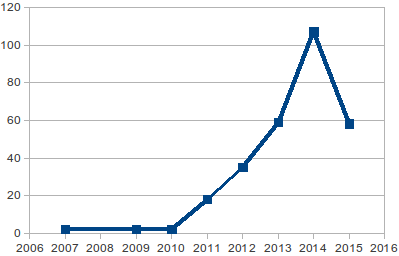
\includegraphics[scale=0.5]{./figs/searchSCOPUS-MAS-SG.png}
	\caption{Number of papers involving MAS and SG \label{fig:searchMASSG}}	
\end{figure}

In particular, the MAS paradigm can be adapted to model, control, manage or test the operation of MG. 
The latter had become a basic and fundamental infrastructure in the SG environment and have been receiving attention in recent literature works \cite{Olivares2014TrendsMG},
being envisioned as a possible future energy system archetype \cite{JimenoArchitectureMG2011}.
As noticed by Jiayi, Chuanwen \& Rong \cite{Jiayi2008}, MAS technology can be applied over it in order to assist different operational problems, such as:
connecting small Distributed Energy Resources (DER) units, coordinating several local decisions;
providing tools for MG in order to operate in a liberalized market of energy trade;
promoting stability and high quality energy for its local environment.
With MAS, each control unit in a MG (e.g., DG, DS, or load controller) is designed as
an agent \cite{Dou2014}, and  its operation is determined by
devices interaction through intelligent decision making process and collaborations of these agents.

MG systems aggregate many DER and loads together as an autonomous entity \cite{Zheng2010}.
Furthermore, additional components added by consumers, or sometimes already presented and just integrated to the SG, impose new frontiers for MG control and management.
For example, Plug-in Electric Vehicles (PEV) \cite{Romo2015} are being integrated to the power grid (specially with the rise of smart charging parks, namely SmartPark \cite{Mwasilu2014}),
imposing new grid constraints, requirements and goals, settled by its users. 
Coordination and integration of DER in MG systems have been the focuses of different researches and remain a complex task \cite{Logenthiran2008}.
This integration may cause lack of efficient control and problems in stability, reliability, power quality and security over MG.
Thus, as emphasized by Agrawal \& Arvind \cite{Agrawal2014}, MAS seems to have appealing features meeting operation,
control requirements and goals balance of the entities that integrate the MG systems.
Figure \ref{fig:searchMASMG} shows the number of publications linking MAS and MG.

%power generation paradigm is going green by involvement of renewable energy sources

\begin{figure}[htbp]
\centering	
	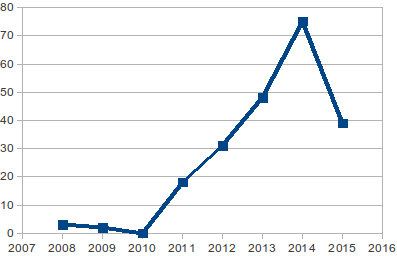
\includegraphics[scale=0.5]{./figs/searchSCOPUS-MAS-MG.png}
	\caption{Number of papers involving MAS and MG \label{fig:searchMASMG}}	
\end{figure}

This field has not been researched only by academics,
patents have been requested related to MAS applications \cite{goldsmith2012computingPatent, SAMPIGETHAYA2012}.
Goldsmith \cite{goldsmith2012computingPatent} registered a patent, deposited in the end of 2011, 
for a MG encompassing a geographic range of less than 300 square miles,
comprising less than five thousand different power sources and less than one hundred thousand different loads.
They described a computing architecture that facilitates autonomously controlling operations of a MG.
Encompassing a computing device being a portion of a decentralized, distributed network, wherein computing devices in the decentralized, 
distributed network perform computations using MAS technologies. 
 
As can be seen, many works in the literature adopt an agent based solution to implement
intelligence communication and optimization over the emerging smart electric grids.
However, Sanz, Rodrigues, Soler \& Gallejo \cite{Gomez2014ReviewMGFromMASUse} pointed some misunderstandings in
the way agent based systems are  being applied to MG systems, such as: 
consideration of one instance of each agent type; 
agents without really decision capabilities; 
components distribution but only decentralization; 
agent interaction is a client-server one instead of peer-to-peer.
On the other hand, new research fields involving MAS are evolving from SG applications, Figure \ref{fig:HAM-HCF} shows
a hybrid multi-agent control model, so-called HAM, proposed by Dou et al. \cite{Dou2014}.

\begin{figure}[http]
\centering
	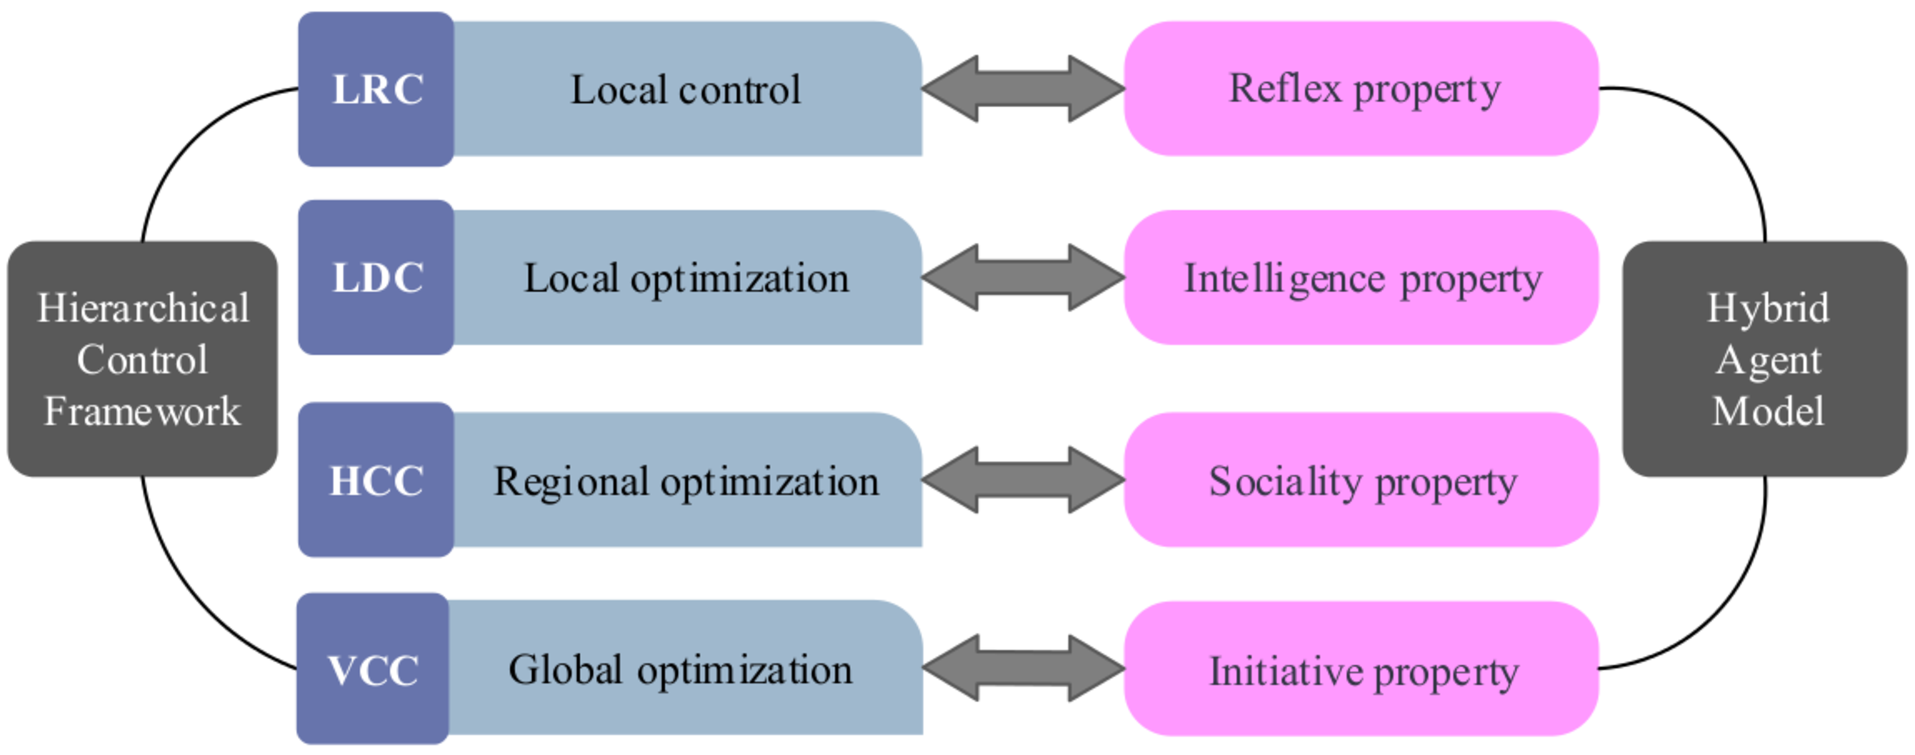
\includegraphics[scale=0.3]{./figs/HAM-HCF-relation.pdf}
	\caption{Relations between hybrid multi-agent control model (HAM) and hierarchical
control framework (HCF). \cite{Dou2014}  \label{fig:HAM-HCF}}	
\end{figure}

Integrating these emerging hybrid tools in order to assist SG viability is 
the most important task tackled by the researchers.
Our current work will discuss about what has been done in this field with
a main focus on MAS state-of-the-art applications over MG.
We will present some trends and prospectives envisioned by us and also extracted from the literature.
%Different distributed management solutions based on the paradigm of MAS applied to smart-microgrid are analyzed in this survey. 

Section \ref{sec:MASSGControl} describes applications related to MAS and coordination, control and management of SG components.
Section \ref{sec:MASSmartMG} presents an overview of MAS and smart-microgrid systems.
Decentralized approaches for MG operation and management are presented in Section \ref{subSec:MASMGSmartControl}.
Section \ref{subSec:MGSecurityAndStability} focuses on MAS and MG in the context of promoting SG security and grid stability.
The of state-of-the-art regarding to stand-alone MG managed by MAS is explored in Section \ref{subSec:standAlone}.
Energy storage systems are discussed in Section \ref{subSec:MASESS}, 
demand control system are presented in Section \ref{subSec:MASDemandControl}, 
Section \ref{subSec:SGServiceRestoration} reviews some applications related to Power Distribution System Reconfiguration (PDSR),
focusing on service reconfiguration problems.
Section \ref{sec:futureApplication} introduces some future applications expected between MAS and the field of Smart-Microgrids.
Finally, some conclusions are drawn in Section \ref{sec:conclusions}.


\section{MAS and SG  \label{sec:MASSGControl}}

The term Smart Grid has been more oriented to the entire electrical system including generation, transmission and distribution \cite{Ekanayake2012BookSG}.
Regarding the distribution system, several efforts target the increase of manageability and efficiency by dividing the 
smart distribution grid into sub-systems. 
Figure \ref{fig:SGFutureVision} presents a future vision of a SG, adapted from European Commission report on SG \cite{SGVisionReportEuropeanComission2006}.

\begin{figure}[http]
\centering
	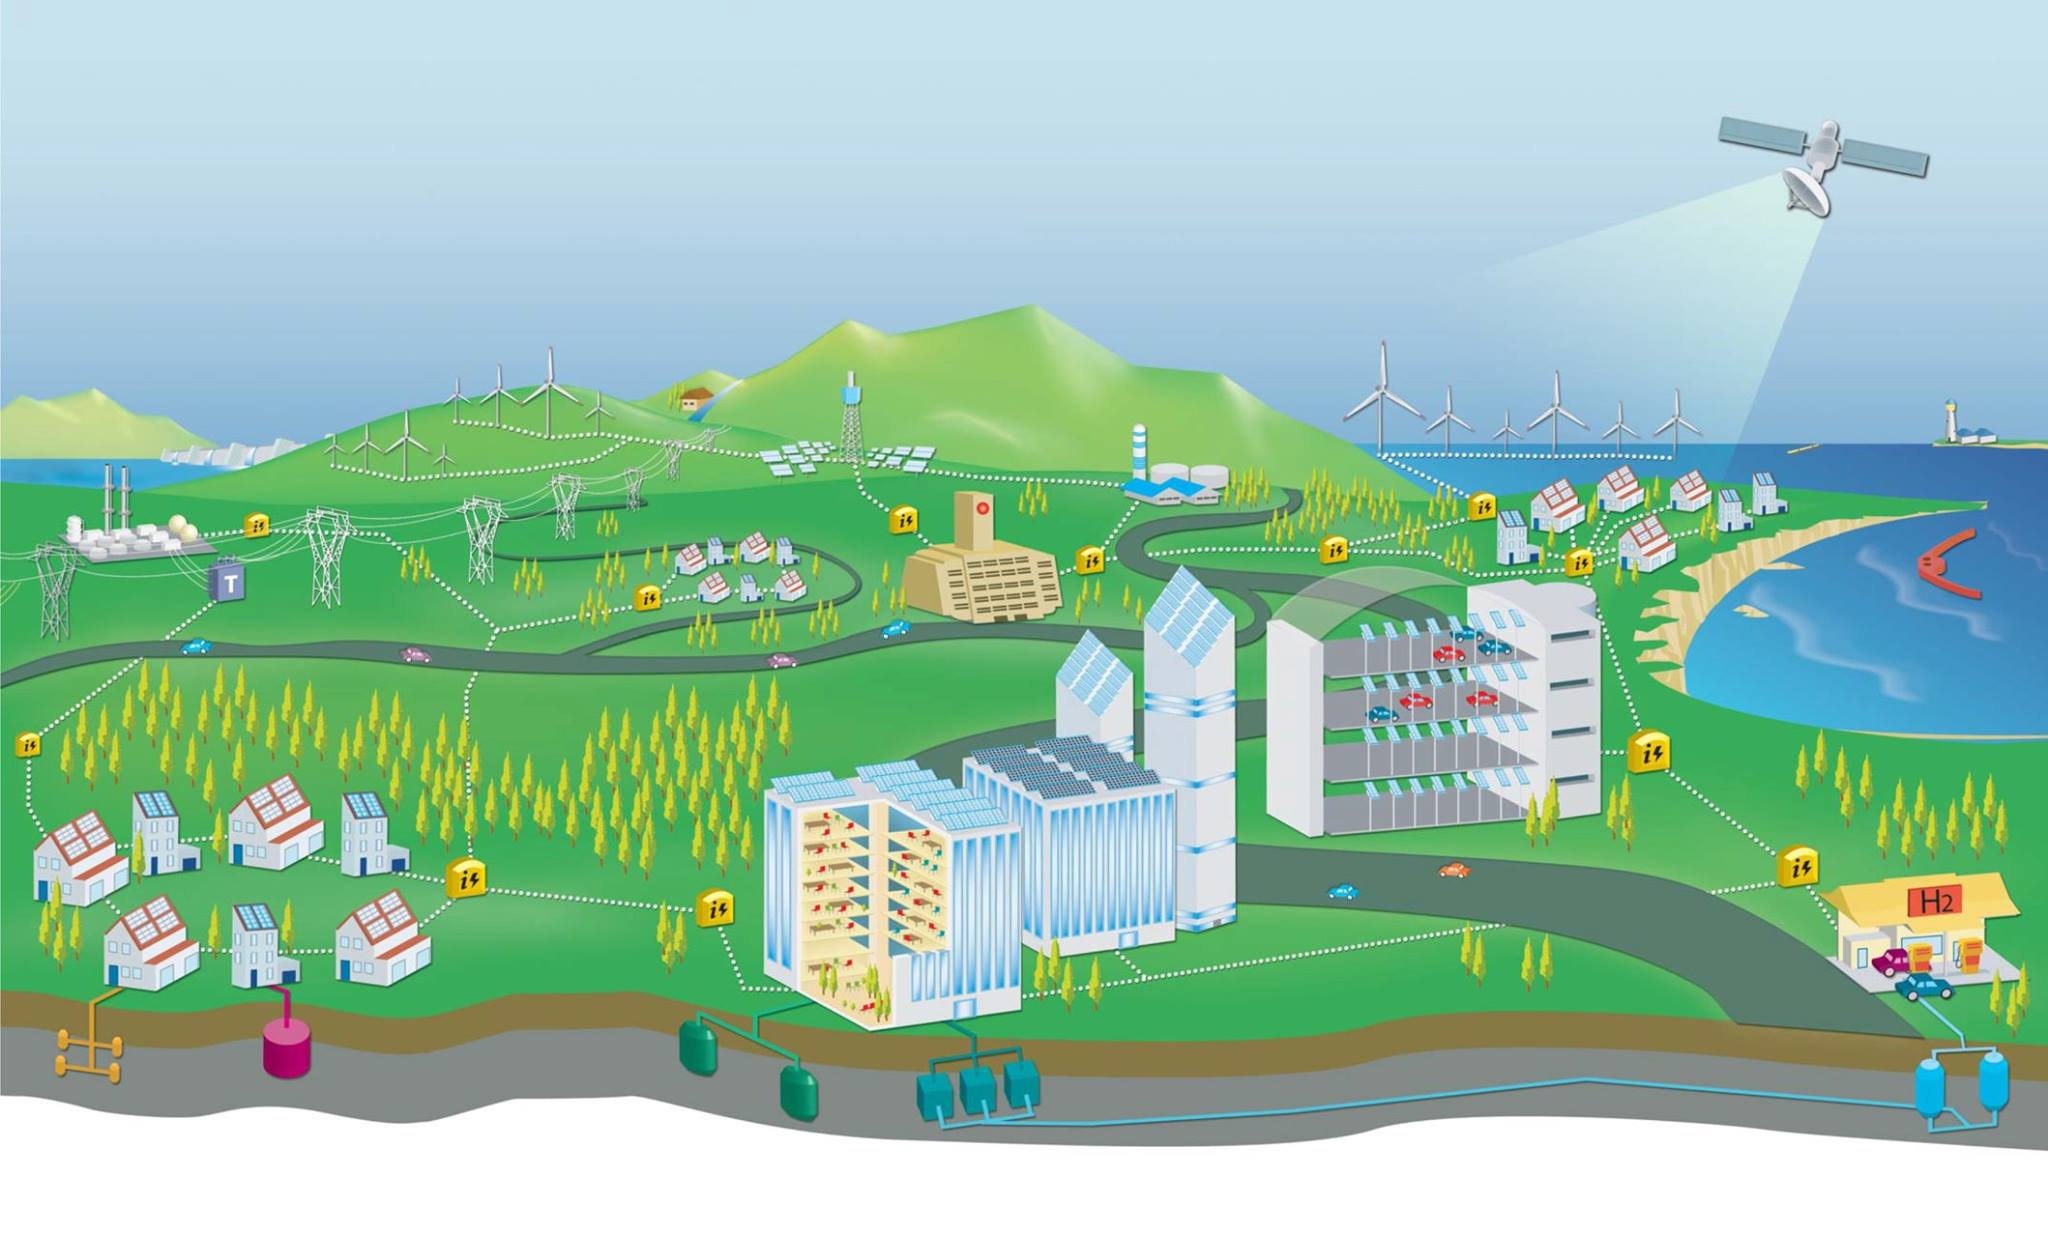
\includegraphics[scale=0.14]{./figs/smartGridFutureVision.jpg}
	\caption{Adaptation from the Future Network Vision of European Commission report on SG \cite{SGVisionReportEuropeanComission2006}  \label{fig:SGFutureVision}}	
\end{figure}

Different sub-systems will compose the future SG, as can be imagined through Figure \ref{fig:SGFutureVision}.
These sub-systems are called ``Smart-Microgrids'', or just ``Microgrids'', 
and consist of energy consumers and producers at a small scale, which are able to manage themselves, being self-sustainable or in stand-alone state.
The environment depicted involve different components idealized for the future power grids, such as: 
Hydro power stations (medium and small); Low emission power plants; Solar power plant;
Biomass;  Wave energy generation (a brief view of these last five RER can be seen in Ellabban, Abu-Rub \& Blaabjerg \cite{Ellabban2014});  
Offshore wind farms \cite{Ederer2015Offshore};
Residential photovoltaic generation;
Batteries bank (Battery Energy Storage System \cite{Levron2013}, Compressed Air Energy Storage systems \cite{Manchester2015RegenerativeAirEneStorage},
Flywheels \cite{RigoMariani2014}, Thermal Energy Storage \cite{Comodi2015}, Pumped-storage hydroelectricity \cite{Zakeri2015}, 
Superconducting Magnetic Energy Storage \cite{tinador2008superconducting});
PEVs \cite{GarciaPEVReview2014};
Distribution and management: Transformers, HVDC link, underground systems and power transmission, control and communication center and satellites.
Small wind turbine on buildings rooftops \cite{Tabrizi2015} and Smart Parks \cite{Kumar2014WCCI} could be also envisioned for this future system. 

The choice of RER by the future power grid is being expected, 
and this growth is also motivated because of the need of reducing environmental impacts, as emissions of greenhouse gases \cite{PereiraJr2013,Welsch2013}.
The potential for RER is growing quick and it is expected that it will, in principle, exponentially exceed the world's energy demand \cite{Ellabban2014}.
SG infrastructure should also provide new opportunities for the grid and its customers for 
information exchange regarding real-time electricity rates and demand profiles \cite{Kahrobaee2014}.
The massive insertion of these RER motivates the development of management systems able to integrate these DER to the SG.

%Energy management system of SG is tightly associated with the communications between stakeholders and entities. 
%Providing essential infrastructure for consumers and stakeholders to monitor and control their energy production and usage should be taken into account over the new systems.

Studies in the field of DER management usually request the inclusion of criterion such as fault tolerance and adaptability.
Lagorse, Paire \& Miraoui \cite{Lagorse2010} reported that the designer of the components of these systems generally knows each agent response separately.
Centralized management system focuses its attention solely on the overall reaction of the system.
Thus, the use of a paradigm based on MAS has been showing to be reasonable.

Brown \cite{Brown2008} emphasized bidirectional communication between devices as the most important characteristic for integrating new DER into the energy systems. 
From this communication process and standards (for example IEC61850, as can be seen in Figure \ref{fig:MASSystemZhaoAltitude}, or ZigBee based protocols \cite{Batista2013}), 
a process of decision making is taken by different SG components.
In this sense, the convenience for new MAS applications using agent peer-to-peer interaction instead of client-server will 
face an open field in the next years.
The migration to this new business model and the implementation of the SG 
has as its starting point the installation of Smart Meters (SM) \cite{McHenry2013}, which improve access to electricity consumption information,
and sensors in residences or commercial buildings.
SM are a key enabler for communication between SG devices.

The IEEE Power and Energy Society addressed the existence of agent research in the rising SG through two reports.
McArthur et al. \cite{McArthur2007a} advocated the interest in investing in agent technology for Power Grids, 
concluding that a MAS could be used either as a way of building robust and flexible hardware/software systems or as a modeling approach. 
A second report done by McArthur et al. \cite{McArthur2007b} emphasized techniques and tools that could allow engineers to use MAS.
They also recognized the Java Agent Development Framework (JADE) \cite{Bellifemine2001JADE}, which is a FIPA (The Foundation for Intelligent
Physical Agents) standard-based MAS framework supporting multi-agent development with facilities of agent management, 
as a main agent platform implementation (which is being extensively used in the literature \cite{Wu2014, Yu2015}).
MAS guidelines implementations were discussed and claimed by Sanz, Rodrigues, Soler \& Gallejo \cite{Gomez2014ReviewMGFromMASUse}.

A common consensus is that intelligence over MAS can be implemented by the incorporation of known AI techniques,
such as: Evolutionary Computing, Population based and trajectory search Metaheuristics, Neural networks, Multi/Many-Objective Optimization techniques, among others.
MAS are used as distributed AI tools that, differently from classical AI, 
underpins its research on the possibility of learning from  social phenomena \cite{Wooldridge2009MASIntroduc}.
They are often cited as the evolution of distributed control \cite{Karfopoulos2015},
where two or more physical or virtual (software) entities interact with each other, capable of tackling
sub-problems in order to reduce complexity of the main problem.
MAS have been applied to regulate, coordinate and control SG, as will be presented throughout this work.
The involved entities are namely agents. 
Some common properties found over these agents can be found in several MAS applications in the field of SG \cite{Logenthiran2011, Dou2014, Karfopoulos2015}.
An interesting distributed cognitive agent modeling architecture was reported by Velik \& Nicolay \cite{Velik2014}, even it was not applied into a MAS 
many characteristic applicable in distributed models can be extracted from their work.
A flowchart can be seen reproduced in Figure \ref{fig:genericAgenteArchitetura}, and some properties of MAS and its agents are highlighted below:

\begin{itemize}
\item Flexibility -- the MAS structure allows advanced plug-and-play capabilities and adaptively adjust the control of
MG according to actual conditions and targets. 
Agents are able to present self-adaptive behavior in accordance to the environment 
and act accordingly in order to accomplish their personal goals (mono or multi objective functions).
\item Fault-tolerance -- if one agent fails, 
the role system remains communicating and able to adapt its new states admitting previous established rules and behaviors.
Thus, control of individual DGs is robust to disturbances and faults in the context of MG. 
\item Autonomy -- the ability to operate in order to attend specific and individual objective functions
and also being guided by a global communitarian goal, without constant guidance from the user side.
\item Responsiveness: 
collect environment information, data base (Figure \ref{fig:genericAgenteArchitetura}) or real-time data acquisition, and completing a decision making process provide
agents the ability to respond to changes.
\item Pro-activeness -- the ability to reason and initiate its own actions in order to meet its specific objectives, 
sometime guided by its own beliefs (i. e., by processing information from deterministic or probabilistic forecasts \cite{Hong2014,Zhang2014,Weron2014}).
\item Social ability -- the ability to bargain, collaborate, compete and exchange knowledge with other virtual or physical agents.
\item Scalability -- extend and expand the functions of a MAS based on SG users' needs is feasible and suitable.
\end{itemize}

\begin{figure}[http]
\centering
	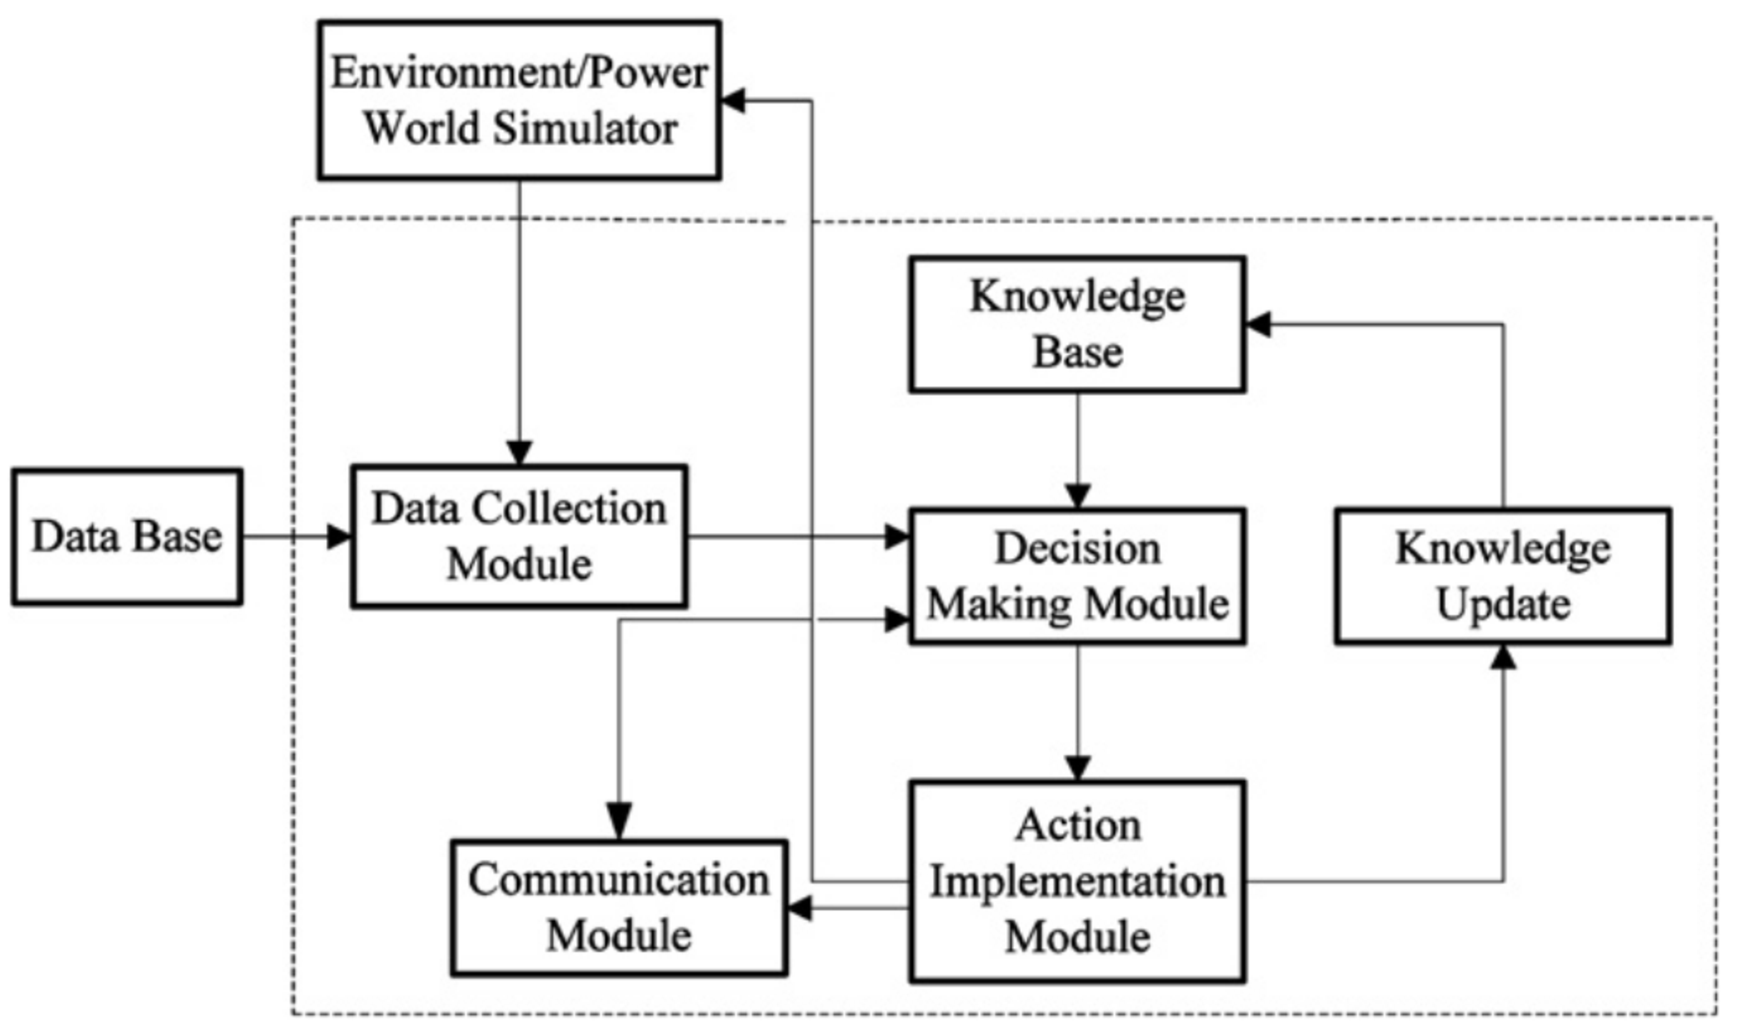
\includegraphics[scale=0.4]{./figs/genericAgenteArchitetura.pdf}
	\caption{Agent architecture. \cite{Logenthiran2011}  \label{fig:genericAgenteArchitetura}}	
\end{figure}

\section{MAS and Smart-Microgrids \label{sec:MASSmartMG}}

%Stafell \& Green \cite{Staffell2014} discussed how does wind farm performance decline with age and they verified that onshore wind farm output falls 16\% a decade, 
%possibly due to availability and wear.
%offshore wind farms  was considered reasonable alternative energy sources for SG system by Ederer \cite{Ederer2015Offshore}.


Making electricity grids smarter is a challenging, long-term, and ambitious process.
There is a broad consensus of the necessity for smarter microgrids;
yet, stakeholders also associated a range of risks and barriers such as lack of investment, 
disengaged consumers, complexity and data privacy with measures to make the grid smarter.
They are implicit motivating the growth of MG,
since stakeholders felt many smart energy system functions are more likely to be implemented in urban areas \cite{Xenias2015}.
Rendering the situation even more complex,
more people are expected to still keep moving to urban areas, especially in developing countries \cite{Almulali2013}.

Complex smart-microgrid environments are been quoted for RER implementation, such as green roofs \cite{Saadatian2013}.
Tabrizi, Whale, Lyons \& Urmee \cite{Tabrizi2015} pointed out that installation of small wind turbines in rooftops is 
not only feasible but also suggested by architects and project developers.
This choice is a potential innovative way for incorporating sustainable energy generation into building design.
Efforts in the context of improving wind energy production in urban areas were also pointed out by Ishugah, Li, Wang \& Kiplagat \cite{Ishugah2014},
and also technical works aimed at improving its use in turbulent urban wind environment \cite{TojaSilva2013}.
Sarralde, Quinn, Wiesmann \& Steemers\cite{Sarralde2015} discussed solar energy and urban morphology. 
Scenarios for increasing the renewable energy potential of 4718 neighborhoods in London were analyzed.

As can be seen, incorporation of RER into urban and everyday scenarios has being investigated.
The task of making this decentralized MG smarter involve several challenges and sub-problems,
some of them are being tackled by the use of MAS and will be discussed from now on.

\subsection{Smart-microgrid operation and management  \label{subSec:MASMGSmartControl}}

Effective energy management is a key to achieve vital efficiency benefits \cite{Lopes2006}.
Sanz, Rodrigues, Soler \& Gallejo \cite{Gomez2014ReviewMGFromMASUse} suggested a guidelines to be followed when designing an agent system to manage MG.
An illustrative example using the agent technology IDAPS \cite{Pipattanasomporn2009}, Intelligent Distributed Autonomous Power Systems, to MG was adapted 
and evaluated trough an alternative design, called INGENIAS IDAPS or I2DAPS. 
INGENIAS \cite{Pavon2003INGENIAS} is an Agent Oriented Methodology and it is supported by the INGENIAS Development Kit.

A pioneer research done by Dimeas \& Hatziargyriou \cite{Dimeas2005} 
proposed optimization tools for internal operation MG interacting with the energy market.
Their approach took use of three distributed types of distributed controller, as exemplified in Figure \ref{fig:controlLevelsDimeas},
and modeled four kinds of agents: production agent, consumption agent, power system agent and a coordinating agent.
Every DER was designed for optimizing its own objectives while taking into account the overall benefit through an auction algorithm,
whereas production units could accept or decline a load offer.

\begin{figure}[http]
\begin{center}
\centering
		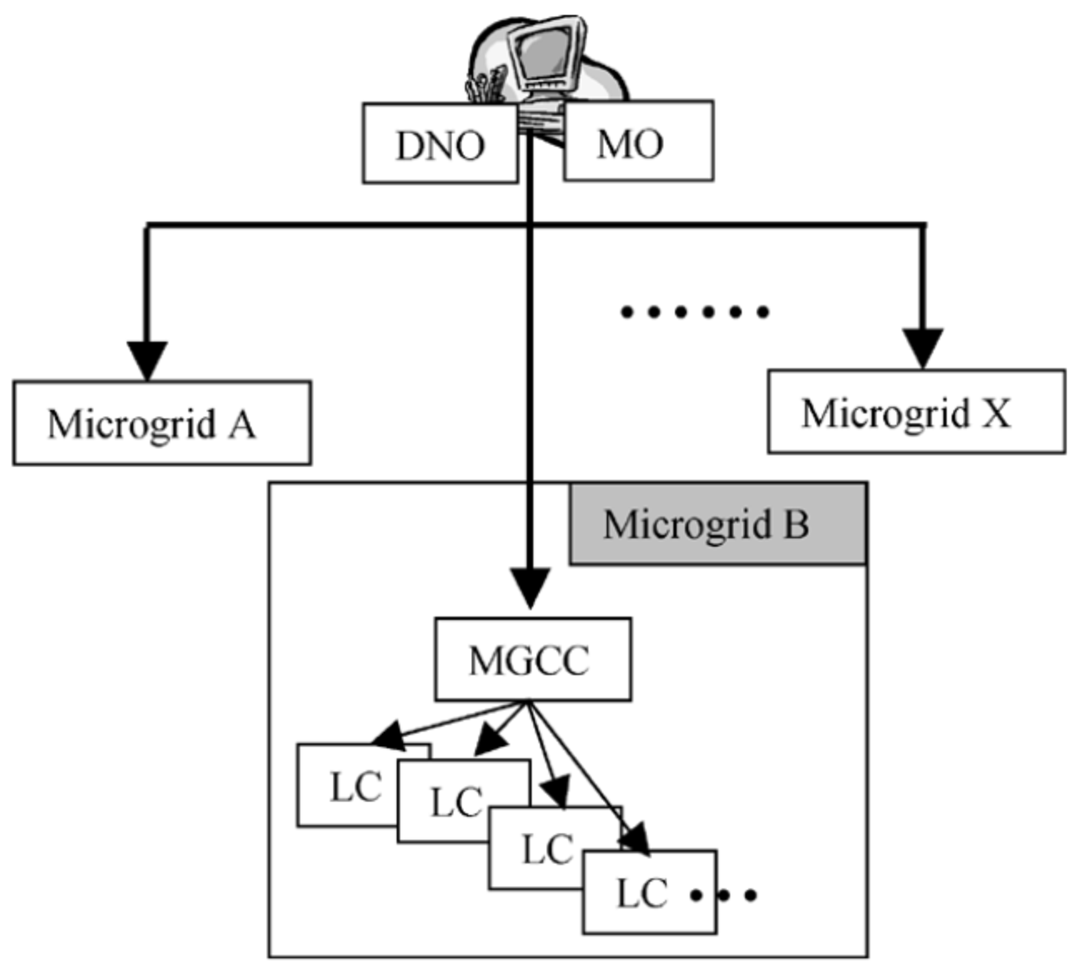
\includegraphics[scale=0.4]{./figs/controlLevelsDimeas.pdf}
\end{center}
\caption{MG control based on three decentralized controllers. \cite{Dimeas2005}. \label{fig:controlLevelsDimeas}}
\end{figure}

A distributed agent based solution to energy management was presented for hybrid energy generation system in Jun, Junfeng, Jie \& Ngan \cite{Jun2011}.
A MG composed of a train station, wind power plant and district was investigated in Kuznetsova, Li, Ruiz \& Zio \cite{Kuznetsova2014}.
An optimization tool was applied to solve goal-directed actions planning of each agent, based on robust optimization concepts.
Their framework showed to be able to improve system reliability and decreases power imbalances.

Other approaches focused on the MG management issue ensuring energy supply with high security and quality control, as recently done by Dou \& Liu \cite{Dou2014}.

%A gas turbine power plant energy control and management was done with MAS by Roche, Idoumghar, Suryanarayanan, Daggag, Solacolu \& Miraoui \cite{Roche2013}.


\subsection{MG security and stability \label{subSec:MGSecurityAndStability}}

Agrawal \& Arvind \cite{Agrawal2014} defined that MG controls should insure connectivity to the main grid or self-isolation.
The transition between these two states should happen, in a rapid and seamless fashion.
The role of switching a MG between island mode to grid-connected mode (vice-versa) is a challenge matter and 
its feasibility was already evaluated through applications of related to hierarchical MAS \cite{Xiao2010,Dou2014HybridMASMGControl}.

The problem of archiving a stable frequency spectrum in MG under islanded operation won particular attention recently \cite{Liu2013MASFrequencyStabilizationIslanded}.
Maintain a specific frequency in the islanded mode as an important requirement,  
the control of DGs' output and charge action of DSs are used in supply surplus conditions and load-shedding and discharge action of DSs are used in supply shortage conditions. 
Kim, Kinoshita, Lim \& Kim \cite{Kim2010LoadSheddingMAS}
proposed a MAS for load-shedding, which is intentional reduction of electricity use, is a critical problem in islanded MG operation based on the MAS.

A multi-agent based protection framework was proposed to enhance the stability of smart grids in Rahman, Mahmud, Pota \& Hossain \cite{Rahman2015MASTransientStabilitySG}.
In Rosa, Silva \& Miranda \cite{daRosa2012}, 
a MAS technology-based platform was considered as potential applications in management and simulation processes for power grids.
Physical grid parameters and network constraints that can be abstracted to MG were considered by the last two mentioned works.

\subsection{Stand-alone smart-microgrids \label{subSec:standAlone}}

Stand-alone MGs have been considered as an efficient way being
standardized for providing electricity in remote areas.
Generally composed with RER and battery storage, 
this systems are playing an important role in solving power supply problems in remote areas such as islands \cite{Zhao2013OperationStandAloneMG}.

In the example presented in Figure \ref{fig:MASSystemZhaoAltitude}, 
Zhao, Xue, Zhang, Wang \& Zhao \cite{Zhao2015} defined seven types of agents for a stand-alone PV-small hydro hybrid MG.
In their proposal, a small-hydro generation plant is controlled by the Frequency regulation agent (FRA), 
diesel generators are controlled by the Dispatchable DG agent (DDA), 
the PV system is controlled by the Intermittent DG agent (IDA), 
the BESS is controlled by the Energy storage agent (ESA), 
and the controllable loads are controlled by the Demand management agent (DMA). 
Thus, individual agents were implemented according on their defined tasks (forecasting ability, frequency control, among other)
and the characteristics of the systems/devices that they were designed for.
Coordination agents Schedule agent (SA) and Operation agent (OA) were the central rule decision makers following a client-server procedure.

\begin{figure}[http]
\begin{center}
\centering
		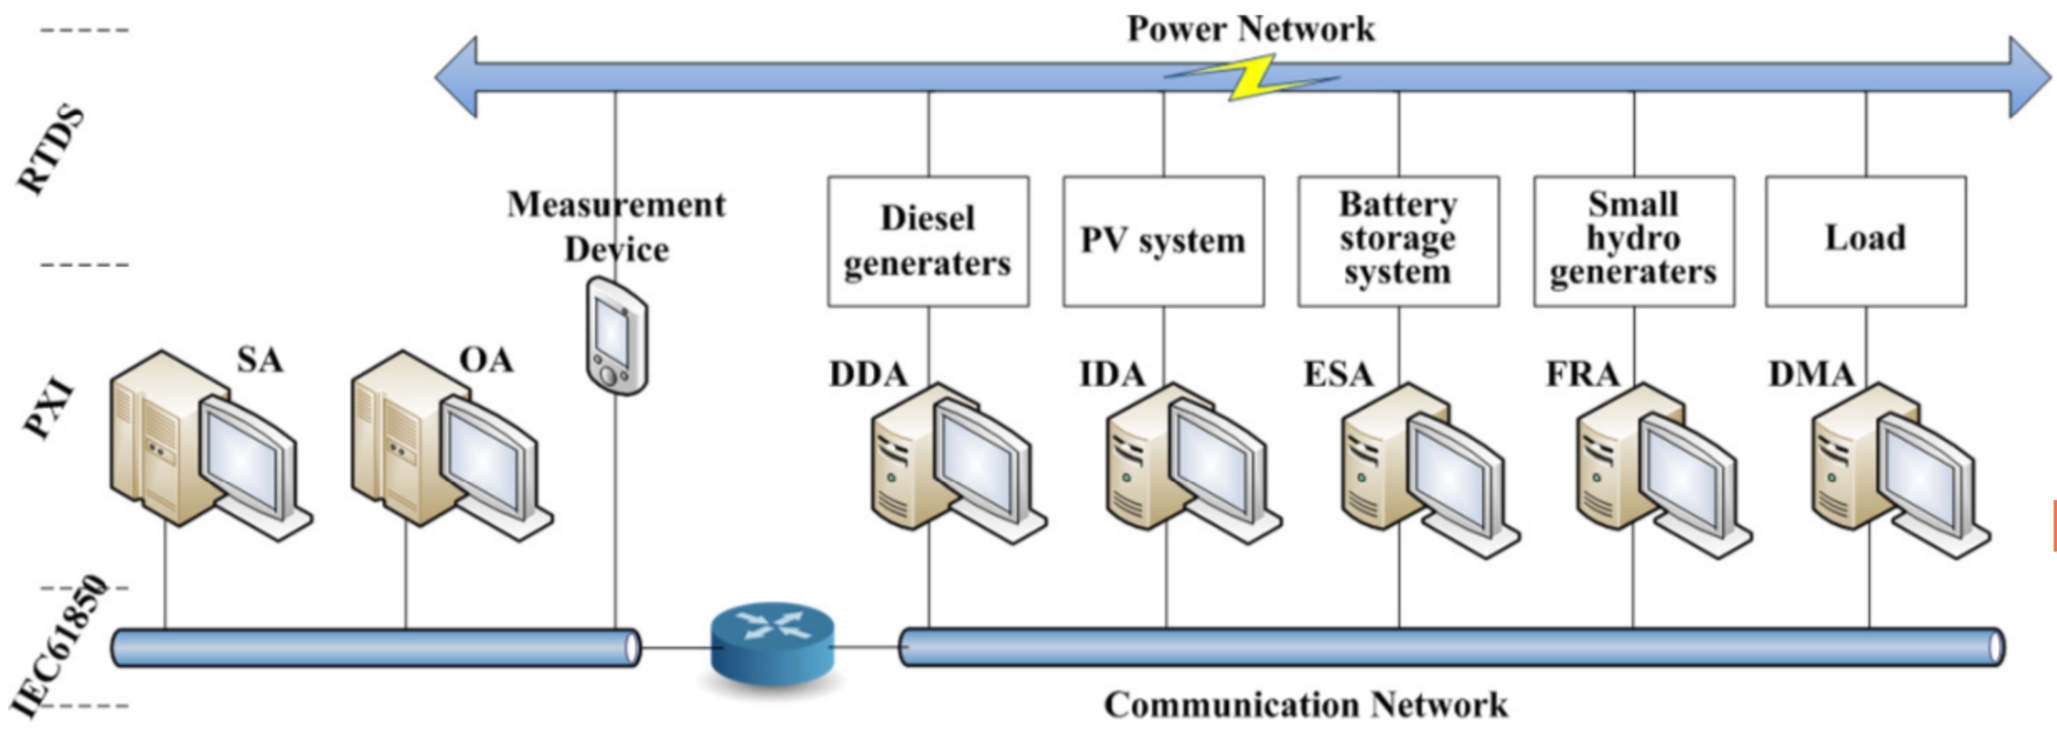
\includegraphics[scale=0.3]{./figs/MASStandAlone.pdf}
\end{center}
\caption{Real-time PXI-RTDS MAS simulation platform for a PV-small hydro hybrid microgrid \cite{Zhao2015}. \label{fig:MASSystemZhaoAltitude}}
\end{figure}

\subsection{Energy storage  \label{subSec:MASESS}}

Energy storage have been widely analyzed for MG systems,
a spread range of applications exist for Energy Storage Systems (ESS).
Tan, Li and Wang \cite{Tan2013} refer the following: 
power quality enhancement;assist microgrid in isolated operation;
active distribution systems and PEVs' technologies.
Its use has important benefits, improving dynamic stability, transient stability, voltage support and frequency regulation \cite{Levron2013}.
Furthermore, they can also be applied for minimizing global cost and environment impacts \cite{colson2009ant}.
Current smart-microgrid scenarios may include different renewable energy resources and several types of storage units.

A wide range of applications exist for Energy Storage Systems (ESS) and we are now able to take profit of MAS over it.
Power dispatching problems \cite{RigoMariani2014} including ESS deals with communications of several different 
SG components, such as energy storage devices, DER and forecasting agents.
%MAS application on ESS have been receiving some considerable efforts. 
%pecially, when handling with PEVs as a possible storage unit \cite{Ibri2012}.
PEVs are one of the most viable technologies to achieve the goals of energy saving and 
environmental protection before a breakthrough in battery technology and fuel cell technology \cite{Zhang2015},
its penetration is expected to increase significantly in the next 20 years \cite{Romo2015}.
Bidirectional power flow between PEVs and the grid will become essential \cite{Saber2010} and 
coordinate this new wave of plug-and-play vehicles is a claiming burden.
 
Hu, Saleem, You, Nordstrom, Lind \& Ostergaard \cite{Hu2015}
applied multi-agent technology, designed with hierarchical architecture (coded with a co-simulation environment called JACK), 
for distribution grid congestion management considering the integration of electric vehicles.
They developed a two level hierarchical control method for integrating PEVs into the grid.
PEVs owners and a distribution system operator were the main agents of the test system, 
communication and agreements were facilitated by the introduction a two operator: fleet and the grid capacity market operators.

Ramachandran, Srivastava \& Cartes \cite{Ramachandran2013} described a decentralized controller using MAS in an electricity market framework.
Their goal was to decide optimal charging based hourly charging rate of each EV battery.
A model with customer comfort zone in order to define demand response was considered.

Switch the operation modes of the storage units based on the MAS by using fuzzy-logic-rules, ensuring a secure and reliable energy supply,
was proposed by Lagorse, Simoes \& Miraoui \cite{Lagorse2009}.
The developed control scheme considered batteries state-of-charge limits and the size of charging/discharging currents.
Motivated by this previous work, Yoo, Chung, Lee \& Hong \cite{Yoo2013BatteryControlMAS} 
improved it using a state machine able to respond to the changes in MG environments for controlling the output power of the DERs.

%Figure \ref{fig:MASMGManagementYoo} shows...
%\begin{figure}[http]
%\centering
	%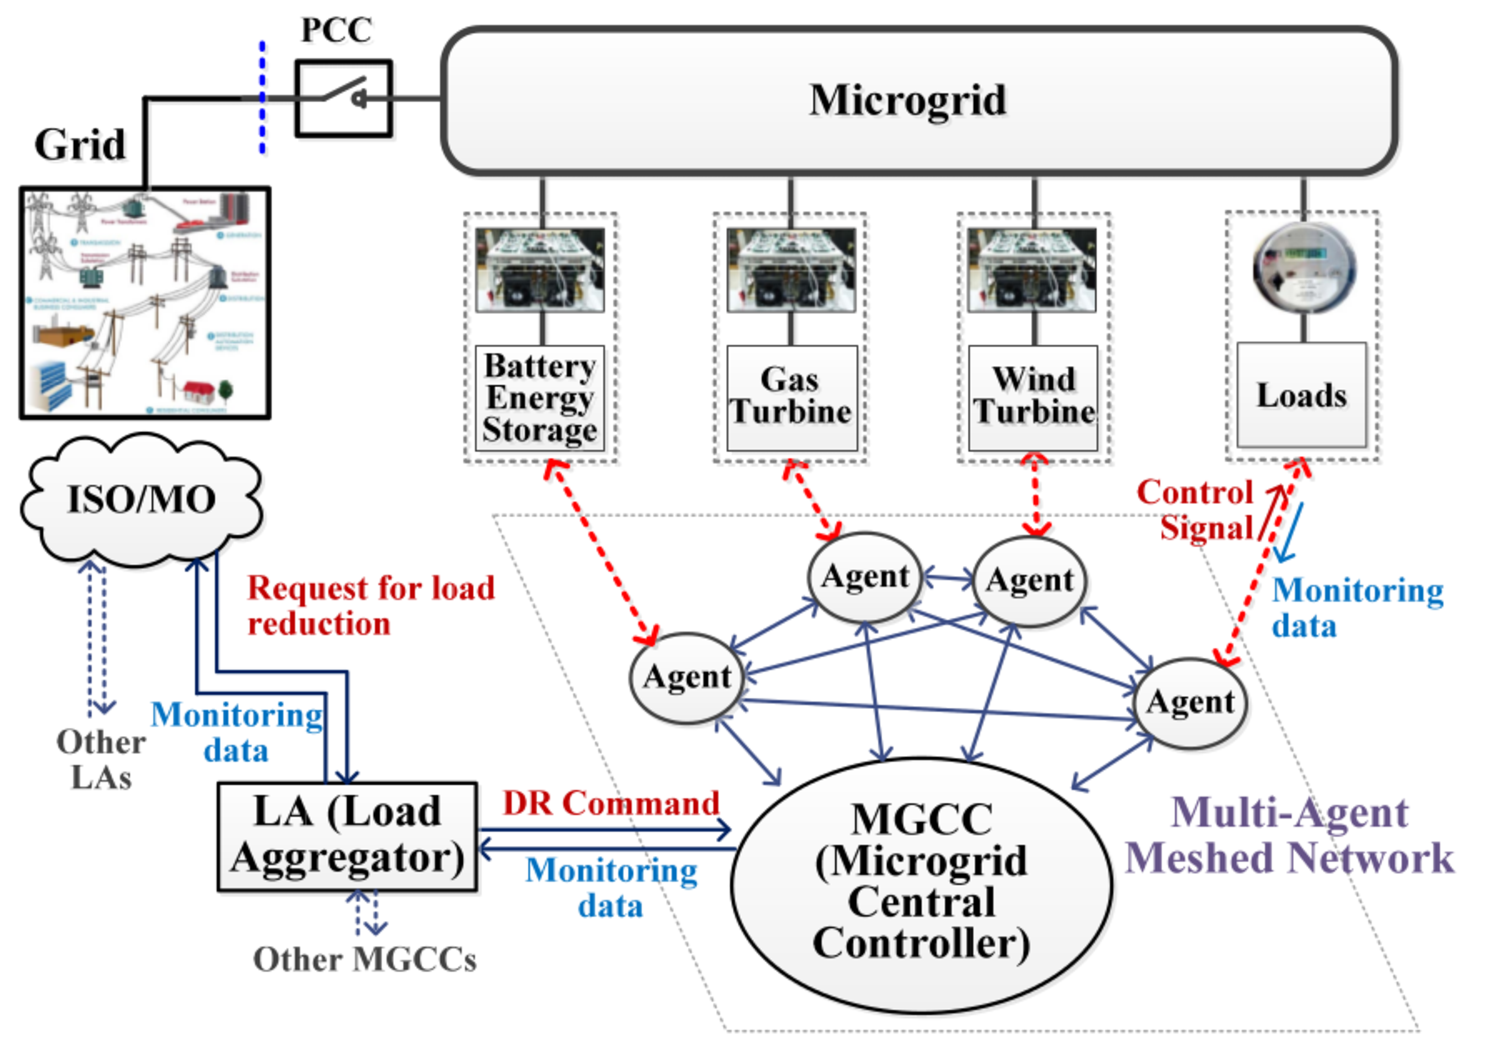
\includegraphics[scale=0.4]{./figs/MASMGManagementYoo.pdf}
	%\caption{Configuration of multi-agent based microgrid energy management \cite{Yoo2013}  \label{fig:MASMGManagementYoo}}	
%\end{figure}

\subsection{Demand control \label{subSec:MASDemandControl}}

Torriti \cite{Torriti2014PeopleOrMachines} remarked that increased awareness regarding consumption should bring about conservation impacts and flatten peak demand.
On the other hand, Sorrel \cite{Sorrell2015} pointed some challenges in reducing energy demand,
due to the strong correlation between increased wealth and increased energy consumption.
Goulden, Bedwell, Rennick-Egglestone, Rodden \& Spence \cite{Goulden2014} discussed the concepts of ''energy consumer`` and ''energy citizen``,
pointing out that we should recognize that SG users are actively engaged with energy, and it is critical to much of what is proposed by demand side management. 
They advocated the contrasting vision is of an active citizen who becomes a ''manager'', a potential MG prosumer.

%MAS application can involve integration of the energy system and mobility-on-demand urban transport systems;

Karfopoulos et al. \cite{Karfopoulos2015} demonstrated MG users satisfaction in household in Spain,
by the use of ICT and operational tools for distributed demand management.
Consumers were intended to participate in grid support without affecting their level of
satisfaction.
A integrated home energy management system enabling the provision of demand response services
from residential customers was proposed,
which was also able to operate under critical/emergency grid operational conditions.

Multi-agent reinforcement learning was used for coordination of consumer agents in a energy management tool proposed by Raju, Sankar \& Milton \cite{Raju2015}.
The consumer was modeled as an agent continuously interacting with the environment and learning how to take optimal actions.
The main goal of the MAS was to achieve the long term objective of reducing total MG power consumption from grid.

Self-demand control building models are been investigated tackling different house components \cite{Zhang2013}.
Smart and energy-efficient building are also the focus of some MAS applications \cite{Smitha2013}, such as building heat distribution control \cite{Mokhtar2013615}.
A multi-agent home automation system for power management was idealized by Abras, Pesty, and Ploix \& Jacomino \cite{Abras2008} and
is an interesting guidelines for this kind of MAS application.
%Machine learning techniques have been contribution for enhancing accuracy in the field of house autonomy
%and data is measured and available for training (Kolter and Johnson 2011)


\subsection{Service restoration \label{subSec:SGServiceRestoration}}

Prado et al. \cite{Prado2014} mentioned the PDSR as a class of SG problems
comprising service restoration, power loss reduction, and expansion planning, which are, nowadays, 
usually formulated as complex multi-objective and multi-constrained optimization problems.
The service restoration problem due to faults has been tackled by several works in the literature.
An example of fault detection and reconfiguration is presented in Figure \ref{fig:serviceRestoration}.

\begin{figure}[http]
\centering
	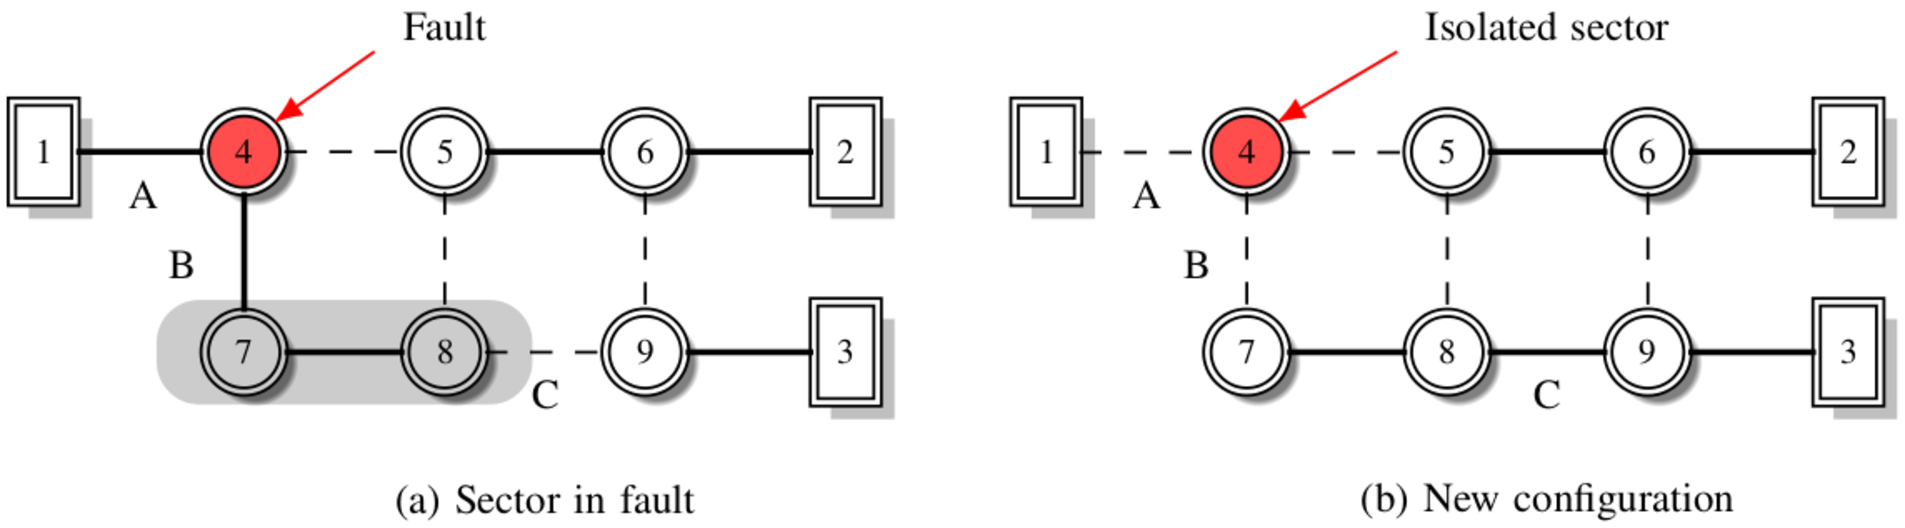
\includegraphics[scale=0.35]{./figs/serviceRestoration.pdf}
	\caption{Power grid service restoration. \cite{Prado2014}  \label{fig:serviceRestoration}}	
\end{figure}

For obvious reasons, SG should be stable and converge in case of any fault or when it falls within the above mentioned problems.
One of the first MAS applications in service restoration was performed in 2000 by Nagata, Watanabe, Ohno \& Sasaki \cite{Nagata2000}, 
consisting in a system with Bus Agents (BAGS) and Facilitator Agent (FAG).
A BAG was developed to decide a sub-optimal target configuration after faults (interacting with other BAGs), 
while a FAG was acting as a manager for the decision process.
Several other works in the literature proposed using the distributed MAS approaches to solve the distribution system service restoration problems \cite{Solanki2007,Pan2009, Yu2015}.

Saraiva \& Asada \cite{Sairava2012MASGerenciamenteTopologica} reconfigured the grid topology in order to satisfy
the operation constraints, according to the data processed by agents dispersed in the grid.

Recently, Yu, Von-Wun \& Tsai \cite{Yu2015} designed switch agents modeled as intelligent agents and organized as local power committees.
Their approach captured the essence of Holonic Multi-Agent Systems (HMAS) \cite{Leitao2009},
which provide self-adaptation and self-organization abilities able to assist management of large and complex systems, such as the case of service restoration in SG.
The local committees were in charge of reaching a consensus among many proposed service restoration solutions after faults were
detected and isolated, as exemplified in Figure \ref{fig:serviceRestoration}.


\section{Future MAS in the context of Smart-Microgrid \label{sec:futureApplication}}

Mariani et al. \cite{RigoMariani2014} tackled the problem of optimal power dispatching in a smart-microgrid scenario
seeking to minimize system total costs.
Mohammadi, Soleymani \& Mozafari \cite{Mohammadi2014} generate a similar scenario considering uncertainties over the forecasting of
consumption and renewable energy generation.
This field of smart power dispatching in MG should receive attention from the next years.
There is a visible lack between state-of-the-art centralized optimization techniques compared to decentralized approaches.
Models that deals with distributed agents might consider uncertainties over agents response or use robust optimization techniques \cite{Kuznetsova2015}.

MAS applications still have an important path in establishing communication between autonomous batteries, specially including PEVs.
Consider constraints and desires regarding to particular batteries (individual agents) in order
to obtain mutual consensus of energy storage remains a challenge problem.
Communication between a main coordinator in order to consider and pondered
the benefit of specific agents in improving grid stability should be discussed and explored in future works.
HCF and HAM system (as described in Figure \ref{fig:HAM-HCF}) could perform a mutual work in finding optimal schedules, 
letting the agents adapt and modify it in real-time.

%In their work, batteries levels was done by using adapting discrete sets of transition levels, around predetermined States of Charge -- SOC, 
%during the space search performed by self-adaptive Dynamic Programming model.
%A study considering metaheuristics based agents in order to calibrate transitions levels between future SOC states can be studied.
%Particularly, strategies intrinsic implemented over each battery of the system,
%could be able to plan the futures SOC levels in real-time, according to a mutual consensus.

Some approaches in the literature incorporated the reduction of greenhouse gas emissions 
as part of a multi-objective optimization problem \cite{Alvarez2009OnlineMinRunningCostCFC, colson2009ant, Kanchev2010SmartMonMG}.
An open field for MAS applications is related to ecological environment monitoring and energy generation \cite{Bousquet2004}.
The potential for SG in contributing to energy sustainability was already discussed by Hu, Li, Cao, Fang, He \& Zhang \cite{Hu2014}.
Agents specialized in improving air quality, water drink-ability, growing of tress and 
several other ecological indicators could can now be weighed on a mutual consensus between MG users and grid managers.

New systems topology of MG including connections to neighbouring MG are emerging and community energy planning has been considered by academics \cite{Huang2015}.
The context of archiving mutual consensus between shared communitarian energy in MG will required specific 
desires set by users and citizens of each neighbor.
Future generations of MAS should be prepared for a scenario with more bargain and distinct objective functions between 
agents from the same class systems (for example, the class of MG users with more marked differences in their goals).

Test MG systems are still being explored and several characteristics can still be sought for optimization and assisted by MAS.
As emphasized by Lidula \& A.D. Rajapakse \cite{Lidula2011TestSystemMG}, 
generic simulation models, reflecting MG properties, are still requested and would facilitate further researches focus on improving transient stability performance, 
system protection, fault tolerance, novel control strategies and standard guidelines designs for MG.

Prado et al. \cite{Prado2014} highlighted that the
performance obtained by metaheuristics applied for service restoration in 
large-scale distribution systems is dramatically affected by the data structures used to represent electrical topology of the power grid system.
In this sense, the need of decentralized approaches for handling service restoration is another open field for researching.
The idea of decentralized power flow calculus could boost the applications of MAS based tools over this class of problems.
More elaborated agents strategies and organizations need to be explored for resolving the system after multiple faults,
solving potentially subtle conflicts.

The grid does not become smarter alone, and yet adding sensors, network nodes with computation capabilities, 
switches or actuators and capability of plug-and-play devices does not make grid smart itself.
As cited by Sanz, Rodrigues, Soler \& Gallejo \cite{Gomez2014ReviewMGFromMASUse}, 
new control algorithms apt to coexist or integrate with standard power management mechanisms are required.
Thus, efforts should be devoted to carefully designing the new SM devices \cite{Pepermans2014ValuingSM} with intrinsic abilities presented in MAS.

Even residential loads are being disaggregated and handled with nonintrusive load monitoring \cite{Perez2014DisagrgregationUsingSM},
MAS applications in the autonomous control of residential houses remains flawed.
These smart decentralized tools would assist householders with better energy consumption management and blaze the trail for efficient autonomous green houses.

\section{Conclusions \label{sec:conclusions}}

According to Ball \cite{Ball2012}: ``There are many arguments for and against the use of autonomous-agents
in ambient intelligence and intelligent environments. Some researchers maintain
that it is vital to restrict autonomy of agents so that users have complete control
over the system; whereas, many others maintain that there is a greater benefit to be
gained by employing autonomous-agents to take some of the work load off the
user and increase user convenience''.

Even the opinions and concerns of people regarding autonomy in SG systems, specially in the context of Smart-Microgrids, 
can differ greatly from person to person, we believe in the flowering of MAS applications for autonomous control for the future power grids.
Such autonomy managed by agents with its own desires and rules, set by MG users and main grid coordinators/managers.

As verified along this paper, it was reported that from operation, management, security and efficient use of resources,
MAS have been studied and, in general, presented feasible and reasonable performance allowing them to be implemented in real-time MG systems.

\section*{Acknowledgment}

The authors would like to thank Brazilian agency CAPES, CNPq (312276/2013-3), 
FAPEMIG (PPM CEX 497-13) and FP7 CORDIS, ``New Horizons for Multi Criteria Decision Making'', for supporting the development of this work.


%Smart grid investments can benefit municipal economic development.
%Stand-alone operational MG, sometimes composed as a communitarian energy resource, 
%are attractive way to eliminate the need of construction of new power lines in remote areas \cite{Man2010}.
%Rogers, Ramchurn \& Jennings \cite{Rogers2012-Challenges} highlighted that demand side, the consumers,
%will have to adapt to the available resources, in contrast to the current model in which the supply should always match the demand.
%Rogers, Ramchurn \& Jennings \cite{Rogers2012-Challenges} discussed three illustrative example using
%MAS over SG. 
%One of the examples focussed on the ability of autonomous agents in learn and model home energy use to assist consumers in the transition to
%time-of-use electricity tariffs.

%Due to the distributed topology of the emerging smart grids system, 
%the paradigm of Multi-Agent Systems (MAS) has been showing an useful tool that has been addressed in different applications. 

% The Smart Grids (SGs) are regarded as the new
% SG. MAS constitute a new field of research in full effervescence
% generation of electric power systems, combining the development and technological development. MAS are particularly useful for
% of Information Technology (IT), distributed systems and Artificial designing distributed systems requiring autonomy of their
% Intelligence (AI) for more features on the real-time monitoring of entities (e.g., bargaining agents, drones, etc.). MAS use new
% the Demand / Response (DR) and the energy consumption
% 


%The use of storage allows both sides, demand and production, to optimize the power exchanged with
%the main grid, in compliance with the electricity market and forecasts.
%Renewable energy generators associated with storage units are considered as active distributed generators, one of
%the fundamental elements of power management in MG systems.

%In this regard, storage is able to increase renewable energy self-consumption and independence from the grid.

% 
% ``The SG components are often distributed and the energy 
% management system is tightly associated with the 
% communications between stakeholders and entities
% (agents) to exchange information. 
% MAS are by nature
% distributed and concurrent, they are independent entities
% engaged in the system, they have their own perception
% of the environment, goal and agenda and they try to
% achieve the best for themselves while behaving strategically. 
% Therefore, in that case when using MAS the amount of data to be disseminated (with its according costs) will be greatly reduced in comparison
% to other in-depth communication methods.''
% 
% SG is a holistic system and the failure of some part of it
% (the breakdown of a transmission line or cut down of a
% substation, transformer. . . .) shouldn't affect the whole
% activities and operations. Flexibility denotes the ability
% of a system to be adaptable (i.e., to behave as required
% in different situations). The flexibility of MAS is given
% by the fact that agents are independent and able to
% perceive their environment and then adapt their actions
% accordingly.
% 
% ``SG should demonstrate the plug-and-play concept for 
% integrating energy storage, loads, and sources at the 
% building level with the external utility grid. Plug and 
% play adaptability is widely proven by MAS, by nature 
% MAS are able to be scaled up by adding other agents or 
% by dispersing them in new environment with new 
% resources and capacities. ''
% 
% As SG will be composed for an aggregate of Microgrid,
% the control can be delegated to micro grids. In this
% vision, the MAS can perform tasks locally if they have
% sufficient knowledge and resources, and they can
% interact with other surrounding agents to help in the
% completion of tasks or decisions. The problem of control
% can be approached from a variety of perspectives
% including cognitive science, heuristic search and
%  machine learning.
%  
%  
%  SG leverage the widespread of the information and
% communication technologies, these smart technologies
% are platform-independent and language free. In this
% perspective, an agent can be developed by a large set of
% languages and communicate with the other agents in the
% system regardless of what language they were programed.



\small

% ACICLOVI

%\bibliographystyle{model1b-num-names}
\bibliographystyle{elsarticle-num}
\bibliography{otimizacao}


\end{document}

